%--------------------
% Packages
% -------------------
\documentclass[11pt,a4paper]{article}
\usepackage[utf8x]{inputenc}
\usepackage[T1]{fontenc}

\usepackage{mathptmx} % Use Times Font
\usepackage{amsmath} % More math

\usepackage{tabularx} % Better tables
\usepackage[pdftex]{graphicx} % Required for including pictures
\usepackage{enumitem} % Includes lists
\usepackage{float} % To make tables work

\usepackage{polski} % Better polish translations (don't use babel!!)

\usepackage[pdftex,linkcolor=black,pdfborder={0 0 0}]{hyperref} % Format links for pdf

\usepackage{calc} % To reset the counter in the document after title page

\usepackage[table]{xcolor} % For colouring tables

\frenchspacing % No double spacing between sentences
\linespread{1.2} % Set linespace
\usepackage[a4paper, lmargin=0.1666\paperwidth, rmargin=0.1666\paperwidth, tmargin=0.1111\paperheight, bmargin=0.1111\paperheight]{geometry} % Margins

\usepackage[all]{nowidow} % Tries to remove widows
\usepackage[protrusion=true,expansion=true]{microtype} % Improves typography, load after fontpackage is selected

\usepackage{lipsum} % Used for inserting dummy 'Lorem ipsum' text into the template


%-----------------------
% Set pdf information and add title, fill in the fields
%-----------------------
\hypersetup{
pdfsubject = {MNiS Projekt},
pdftitle = {Maszyna Boltzmanna},
pdfauthor = {Maciej Obara, Maciej Mak}
}

%-----------------------
% Change caption names
%-----------------------
\renewcommand{\figurename}{Rysunek}
\renewcommand{\tablename}{Tabela}

%-----------------------
% Proper equasions numbering
%-----------------------
\numberwithin{equation}{section}

%-----------------------
% Define colours
%-----------------------
\definecolor{lightlightgray}{gray}{0.90}

%-----------------------
% Titlepage
%-----------------------
\title{Maszyna Boltzmanna - symulacja układu}
\author{Maciej Obara, Maciej Mak}

%-----------------------
% Begin document
%-----------------------
\begin{document}
    \maketitle
    \tableofcontents
    \newpage

    \section{Wstęp}
    \paragraph{Ograniczona maszyna boltzmanna}
    to sieć neuronowa oparta w pewnym stopniu na prawdopodobieństwie, składająca się z 2 warstw;
    \textit{warstwy widocznej}, której wartości są znane i ustawiamy je samodzielnie oraz z \textit{warstwy ukrytej}
    czyli wartości których nie znamy i próbujemy nauczyć tą sieć. Dodatkowo przy każdej
    aktywacji takiego neuronu dodawana jest \textit{jednostka odchylenia}, która jest
    stała dla każdego wejścia.

    \paragraph{}
        Ważną charakterystyką ograniczonej maszyny boltzmanna jest brak komunikacji pomiędzy węzłami na tym
        samym poziomie, każdy węzeł działa niezależnie od sąsiadów, węzeł z warstwy widocznej
        przekazuje swój wynik do każdego węzła z warstwy ukrytej. Pozwala to uniknąć zaburzeń neuronów związanych
        ze klasyfikacją danych wejściowych z innymi danymi wejściowymi. Dodatkowo możemy przez to używać bardziej
        zaawansowanych algorytmów uczenia takich jak rozbieżność kontrastowa.
    \paragraph{}
	    Ograniczoną maszynę Boltzmanna, jak każdą inną sieć neuronową możemy podzielić na kilka etapów
        obliczeniowych. Pierwszym z nich jest znalezienie macierzy wag - trenowanie sieci neuronowej.
        Drugim etapem jest testowanie na postawie innych danych oraz znalezienie odpowiednich cech jakie
        wyróżnił wytrenowany przez nas algorytm. Ograniczona maszyna Boltzmanna pozwala nam równieć szukać
        widocznych neuronów (danych które zwykle wprowadza użytkownik) posiadając tylko neurony ukryte.
    \section{Zastosowania RBM}
    \paragraph{}
        Sieci neuronowe wykorzystywane są do wielu zadań przy których konwencjonalne
        podejście jest mało praktyczne. Jednym z takich zastosowań jest rozpoznawanie
        odręcznego pisma i jego konwersja na dokument tekstowy. Ponadto algorytm taki
        potrafi dostosować się do użytkownika i z czasem rozpoznawać jego styl pisma
        efektywniej i dokładniej. Ma to zastosowanie w tablicach interaktywnych oraz
        smartfonach.

    \paragraph{}
        Najczęściej algorytmy sztucznej inteligencji wykorzystywane są w celu rozpoznania
        jakiegoś schematu w danych które otrzymują. Podczas treningu kontrolujemy dane wejściowe
        w celu nauczenia algorytmu rozpoznawania interesujących nas danych. Ma to szerokie zastosowanie,
        algorytm może rozpoznawać mowę w dźwięku, gatunki zwierząt w zdjęciach, choroby z listy objawów.
	\paragraph{}
	    Do podstawowych zastosowań ograniczonej maszyny Boltzmanna zaliczamy różne metody regresji takie
        jak regresja liniowa czy regresja logistyczna. Innym zastosowaniem tej sztucznej sieci neuronowej
        jest filtrowanie zespołowe, uczenie schematów czy modelowanie tematycze.
    \section{Trenowanie sieci neuronowej}
    \paragraph{}
        Trenowanie sieci neuronowej jest elementem, który ma na celu dopasowanie wag do odpowiednich danych wejściowych.
        Obliczenia dokonują się na podstawie kontrastowej rozbieżności (ang. \textit{Constrastive divergance}), która ma na celu
        dopasowanie wag przez różnice rzeczywistego wyniku działania algorytmu z "wirtualnym" wynikiem wygenerowanym na
        podstawie danych wyuczonych przez algorytm. Całość jest ograniczana przez tzw. współczynnik uczenia, który mówi
        nam o ile algorytm powienien zmniejszyć różnicę otrzymaną z CD. Etap trenowania następuje w określonej liczbie iteracji,
        które w algorytmach sztucznej inteligencji nazywane są epokami
	 (ang. \textit{epochs}).
    \paragraph{}
       Operacje trenowania macierzy najwygodniej przedstawić na macierzach. Za pomocą operacji transpozycji czy mnożenia
       macierzowego można zaoszczdzić sporo czasu na opracowywanie algorytmu RBM. Do treningu będzie potrzebna funkcja sigmoid,
       która przyjmuje wartości od 0 do 1,  a zmiana pomiędzy nimi następuje dla argumentów bliskich zeru.
    \paragraph{}
	 Dodatnia faza kontrastowej rozbieżności jest obliczana za pomocą mnożenia macierzowego danych treningowych i macierzy wag.
	 Wynik tej operacji jest następnie przepuszczany przez funkcję sigmoid, która oblicza prawdopodibieństwo aktywacji danego ukrytego neurona.
    \paragraph{}
	 Ujemna faza kontrastowej rozbieżności jest obliczana za pomocą mnożenia uzyskanych ukrytych neuronów z transponowaną
	 macierzą wag. Wynik tej operacji jest następnie przepuszczany przez funkcję sigmoid, która oblicza prawdopodibieństwo aktywacji
     wirtualnych widocznych neuronów. Nie muszą one być identyczne z naszymi danymi treningowymi.
    \paragraph{}
	 Do aktualizacji wag za pomocą kontrastowej rozbieżności potrzebujemy danych treningowych wymnożonych przez macierz aktywacji
	 oraz macierzy wirtualnych danych treningowych (obliczonych przez nasz algorytm) wymnożonej przez ich macierzy aktywacji.
	 Różnicę tych macierzy mnożymy przez współczynnik uczenia, a każdy element macierzy dzielimy przez liczbę wszystkich wierszy danych treningowych.
    \paragraph{Uwagi}
	 Wektor biasów został tutaj umieszczony wertykalnie oraz horyzontalnie obok macierzy wag.
	 Dzięki takiemu zastosowaniu możemy używać wektora biasów tylko przez mnożenie macierzy oraz jej transpozycję.
	 Dodatkowo biasy są w każdej iteracji poprawiane do wartości 1, żeby nie zostały zaburzone przez operację funkcji sigmoid.
    \paragraph{}
	 Wagi są wybierane losowo. Powoduje to czasami otrzymanie odwrotnych wyników przy następnym testowaniu maszyny.
	 Jednak ze wzlędu na brak warunków początkowych dla wag dla naszego przykładu możemy założyć, że dane testowe są zgodne z losowymi przykładami wag.

    \section{Testowanie sieci neuronowej}
    \paragraph{}
	Testowanie sieci neuronowej jest najłatwiejszym etapem algorytmu ograniczonej maszyny Bolzmanna. Najważniejsze jest, żeby było to przeprowadzone po  		\textit{wytrenowaniu} maszyny przy pomocy danych treningowych. Otrzymany wynik algorytmu jest najbardziej przewidywaną odpowiedzią, która zadowoli 			użytkownika. Testować maszynę Boltzmanna możemy szukając ukryte neurony przy określonych danych testowych lub na odwrót.
    \paragraph{}
	Testowanie jest podobne do początkowego etapu trenowania maszyny boltzmanna. Dane użytkownika w postaci macierzy mnożymy przez wytrenowaną 			macierz wag w celu szukania ukrytych neuronów, lub wytrenowaną, transponowaną macierz wag w celu szukania widocznych neuronów. Następie obliczamy 		zero jedynkowe prawdopodobieństwo na podstawie wyników mnożenia macierzy otrzymanych z funkcji sigmoid. Otrzymane dane są najbardziej zbliżone do 		preferencji użytkownika według zadanych przedtem danych treningowych.
    \section{Wyniki}
    Ze względu na losowość początkowych wag, sieć może zwracać inne wyniki pomimo
    tych samych danych treningowych. Znacząco może różnić się także błąd.

    \subsection{Przypadek 1}
        Najczęściej występujący przypadek, przypisuje wszystkie książki danego autora
        pod warunkiem, że użytkownik polubił przynajmniej jedną:

        \paragraph{}
            Średni błąd wyniósł: $2.7799$. Wykres błędu wygląda następująco:

            \begin{figure}[H]
                \centering

                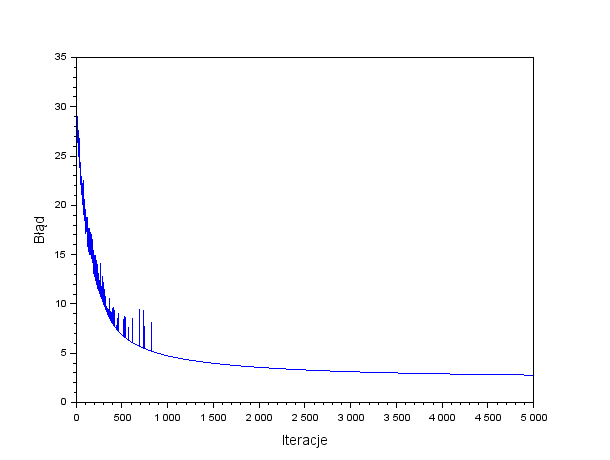
\includegraphics[width=\textwidth]{img/wykres_1.png}

                \caption{Wykres błędu w 1 przypadku}

                \label{rys:1}
                \addcontentsline{toc}{subsubsection}{Wykres \ref{rys:1}}
            \end{figure}

            Widzimy, że błąd w pewnym momencie się ustabilizował i powoli malał.

        \paragraph{}
            Po przeprowadzonym treningu podaliśmy dane wejściowe i przeprowadziliśmy test.
            W danych wejściowych użytkownik podał, że lubi:

            \textit{
                Hobbit, Krew elfów, HP: Kamień filozoficzny.
            }
        \paragraph{}
            Algorytm określił że mogą spodobać mu się:

            \textit{
                Hobbit, Władca Pierścieni, Silmarillion, Historia Śródziemia,
                Krew elfów, Czas pogardy, Chrzest ognia, Wieża Jaskółki, HP: Kamień filozoficzny,
                HP: Komnata tajemnic, HP: Więzień azkabanu, HP: Czara ognia, HP: Książę półkrwi,
                HP: Insygnia śmierci.
            }

        \paragraph{}
            Te wyniki odpowiadają temu czego się spodziewaliśmy, mamy 4 autorów oraz
            4 węzły ukryte, zakładaliśmy że sieć nauczy się rozpoznawać książkę po autorze i
            tak właśnie jest.

    \subsection{Przypadek 2}
        Czasami algorytm nie działa tak jak byśmy się tego spodziewali, w tym przypadku
        widzimy że sieć nie powiązała do końca książek z autorami, jeden węzeł ma pewną
        nieznaną dla nas zależność która zmienia znacząco wynik.

        \paragraph{}
            Średni błąd wyniósł: $3.0233$. Wykres błędu wygląda następująco:

            \begin{figure}[H]
                \centering

                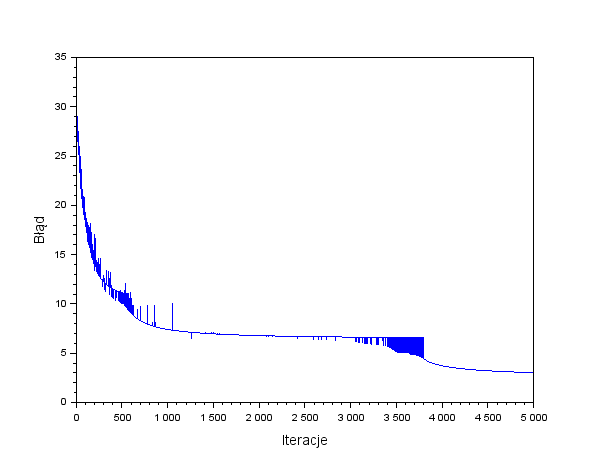
\includegraphics[width=\textwidth]{img/wykres_2.png}

                \caption{Wykres błędu w 2 przypadku}

                \label{rys:2}
                \addcontentsline{toc}{subsubsection}{Wykres \ref{rys:2}}
            \end{figure}

            W tym przypadku błąd się na krótko ustabilizował następnie znowu mocno zmieniał.


        \paragraph{}
            Po przeprowadzonym treningu (na tych samych danych) podaliśmy te same dane wejściowe
            i przeprowadziliśmy test. W danych wejściowych użytkownik podał, że lubi:

            \textit{
                Hobbit, Krew elfów, HP: Kamień filozoficzny.
            }
        \paragraph{}
            Algorytm określił że mogą spodobać mu się:

            \textit{
                Hobbit,  Władca Pierścieni, Silmarillion,  Historia Śródziemia, Przygody Toma Bombadila,
                Uczta dla wron,  Krew elfów,  Czas pogardy,  Chrzest ognia,  Wieża Jaskółki.
            }

        \paragraph{}
            Pomimo tego że użytkownik lubi książkę o \textit{Harrym Potterze} algorytm poleca \textit{Ucztę Wron}.
            W zależności od tego co chcemy osiągnąć jest to działanie niepożądane lub wręcz przeciwnie.
            Ten niespodziewany wynik pokazuje że zawsze trzeba testować swój algorytm przynajmniej kilka
            razy aby móc zaobserwować efekty których nie można przewidzieć.


    \nocite{*}
\bibliographystyle{unsrt}
\bibliography{src/sources}
\addcontentsline{toc}{section}{Literatura}
\end{document}